\documentclass[12pt]{article}
\usepackage[top=1in, bottom=1in, left=1in, right=1in]{geometry}

\usepackage{setspace}
\onehalfspacing

\usepackage[hang,flushmargin]{footmisc} 
% 'hang' flushes the footnote marker to the left,  'flushmargin'  flushes the text as well.

\def\baselinestretch{1}
\setlength{\parindent}{0mm} \setlength{\parskip}{0.8em}

\newlength{\up}
\setlength{\up}{-4mm}

\newlength{\hup}
\setlength{\hup}{-2mm}

\usepackage{amssymb}
%% The amsthm package provides extended theorem environments
\usepackage{amsthm}
\usepackage{epsfig}
\usepackage{times}
\renewcommand{\ttdefault}{cmtt}
\usepackage{amsmath}
\usepackage{graphicx} % for graphics files

% Draw figures yourself
\usepackage{tikz} 

% The float package HAS to load before hyperref
\usepackage{float} % for psuedocode formatting
\usepackage{xspace}

% from Denovo Methods Manual
\usepackage{mathrsfs}
\usepackage[mathcal]{euscript}
\usepackage{color}
\usepackage{array}

\usepackage[pdftex]{hyperref}

\newcommand{\nth}{n\ensuremath{^{\text{th}}} }
\newcommand{\ve}[1]{\ensuremath{\mathbf{#1}}}
\newcommand{\Macro}{\ensuremath{\Sigma}}
\newcommand{\vOmega}{\ensuremath{\hat{\Omega}}}

\begin{document}
\begin{center}
{\bf NE 155, Class 16-18, S14 \\
DE \\ February 28, March 3 and 5 2014}
\end{center}

\setlength{\unitlength}{1in}
\begin{picture}(6,.1) 
\put(0,0) {\line(1,0){6.25}}         
\end{picture}

%-------------------------------------------------------------
I'm going to change the ordering of the syllabus a little bit a drop  a topic. After thinking about it, I think this is overall the best way to go. At the end we'll see if you agree. 

I'm going to skip item \# 3: Point Kinetics and numerical solution of the initial value problem. Instead I'm going to go through a derivation of the transport and diffusion equations more deeply. While this isn't entirely needed, I just feel like it's more satisfying. 

We will then spend a bit more time on the diffusion equation and solution methods (\#4). For the purpose of projects I'm going to switch the ordering of Monte Carlo and Transport Solution methods (\#s 5 and 6). This way you can either do a diffusion solver project or a Monte Carlo project with some information about either method with enough time to do the project. 

Cool?

\section{Transport Equation Redux}

Largely from Lewis and Miller Chp.\ 1 and Duderstadt and Hamilton Chp.\ 4. 

\subsection{Definitions}

Spatial logistics
\begin{itemize}
\item $d\vec{r} = d^3r$ = ordinary volume = $r^2 sin(\theta) d\theta d\phi dr$
%
\item $v$ = speed (scaler)
\item $\vec{v}$ = velocity (vector)
\item $d\vec{v} = d^3v$ = velocity volume = $v^2 sin(\theta')d\theta' d\phi' dr$
\item $v = \sqrt{(2E)/m}$ where $m$ is the rest mass of the particle. Thus, we can relate energy and speed.

\item $\Omega$: unit directional vector in velocity space, $\vec{v} = v\vOmega$
\item $d\vOmega = sin(\theta')d\theta' d\phi' =  d^2\Omega$
%\item thus $d\vec{v} = v^2 dv d\vOmega$
\end{itemize}

\begin{figure}[h!]
\begin{center}
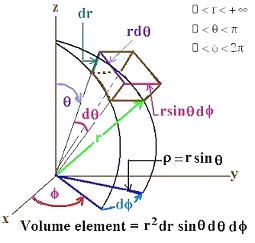
\includegraphics[height=2 in]{VolumeElement}
\end{center}
\end{figure}

Physics terms given possible reactions we're generally going to worry about:
\begin{itemize}
\item total (t): all interactions. Under there there is 
\item scattering (s): a neutron interacts with an atom and bounces off either elastically or inelastically.
\item absorption (a): a neutron is absorbed by a nucleus. If this happens it might
\item fission (f): cause the nucleus to split into 2 pieces, releasing more neutrons
\end{itemize}

\begin{enumerate}
\item \textbf{microscopic x-sec} ($\sigma$, [$cm^2$]): measure of the probability that an incident neutron will collide with a specific nucleus. $\sigma_j$ indicates a specific reaction, e.g.\ $j=f$ is fission.

\item \textbf{macroscopic x-sec} ($\Sigma$ [$cm^{-1}$]): measure of the probability per unit path length that an incident neutron will collide with a target
\[\Sigma_j = \sigma_j N\]
where N is the atomic densigy of the target.

\item \textbf{double-differential scattering x-sec} ($\sigma(E, \vOmega \rightarrow E', \vOmega')dE' d\vOmega'$): measure of the probability that a neutron of energy $E$ and moving in direction $\vOmega$ scatters off of a specific nucleus into energy range $[E', E' + dE']$ and direction range $[\vOmega', \vOmega' + d\vOmega']$.

\item \textbf{fission yield} ($\nu(E)$): is the average number of neutrons released by a fission induced by a neutron of energy E.

\item \textbf{fission spectrum} ($\chi(E)dE$): average \# of fission neutrons produced with energy in $[E, E + dE]$

\item \textbf{particle angular density} ($n(\vec{r}, \vOmega, E, t)d\vec{r} d\vOmega dE dt$): expected number of particles in volume element $d^3r$ at $\vec{r}$ whose energies are in $[E, E + dE]$ and direction of motion is in $[\vOmega, \vOmega + d\vOmega]$ at time $t$

\item \textbf{particle density}: ($N(\vec{r},E,t)d^3r dE$): expected number of particles in $d^3r$ at $\vec{r}$ whose energies are in $[E, E + dE]$ at time $t$.
\[N(\vec{r},E,t)d^3r dE = \int_{4\pi} d\vOmega n(\vec{r}, \vOmega, E, t) \]

\item \textbf{angular flux}: $\psi(\vec{r}, \vOmega, E, t) \equiv v n(\vec{r}, \vOmega, E, t)$ [not a vector]

\item \textbf{scalar flux}: $\phi(\vec{r},E,t) \equiv v N(\vec{r},E,t)$ [not a vector]
\[= \int_{4\pi} d\vOmega \psi(\vec{r}, \vOmega, E, t) \]

\item \textbf{interaction rate density}:
\[\int_{4\pi} d\vOmega \Sigma_j v n(\vec{r}, \vOmega, E, t) = \Sigma_j \phi(\vec{r},E,t)\]
expected number of $j$ reactions per volume per energy at time $t$.

\item \textbf{angular current density}: $\vec{j}(\vec{r}, \vOmega, E, t) = \vec{v} n(\vec{r}, \vOmega, E, t)$ 

Note $\vec{j}(\vec{r}, \vOmega, E, t) \cdot \hat{n} dA dE d\vOmega$ is the expected number of particles crossing $dA$ along $\hat{n}$ with energy in $[E, E + dE]$ and direction in $[\vOmega, \vOmega + d\vOmega]$ at time $t$
\end{enumerate}

%-----------------------------------------
\subsection{Assumptions}
\begin{enumerate}
\item Particles are point objects ($\lambda = h/(mv)$ is small compared to the atomic diameter): its state is fully described by its location, velocity vector, and a given time. This ignores rotation and quantum effects.

\item neutral particles travel in straight lines between collisions.

\item particle-particle collisions are negligible (makes TE linear).

\item material properties are isotropic (generally valid unless velocities are very low).

\item material composition is time-independent.

\item quantities are expected values: fluctuations bout the mean for very low densities are not accounted for.
\end{enumerate}


%-----------------------------------------
\subsection{Derivation}
The TE is a \underline{detailed} balance of the particle population over phase space that is as close to exact as possible. 

Consider a volume $V$ with surface $S$ (draw picture). For each point $\vec{r} \in S$, let $\hat{n}_S$ be the outward normal vector.

For a given $\vOmega$, define $S^+$ as that part of $S$ for which $\hat{n}_S \cdot \vOmega > 0$ (outgoing particles) and $S^-$ as that part of $S$ for which $\hat{n}_S \cdot \vOmega < 0$ (incoming particles).

Then, for a this volume $V$ for a fixed $E$ and $\vOmega$, the general rate equation can be written as 

For particles satisfying $\vec{r} \in V$, energies in $[E, E+dE]$ and direction $[\vOmega, \vOmega + d\vOmega]$:

\hspace*{3 em} Rate of change of the particle (neutron) population 
 = rate of production - rate of loss






If fission is occurring, it is often of interest to know the \textbf{asymptotic behavior} of the system. A reactor is called \textbf{``critical''} if the chain reaction is self-sustaining and time-independent. 

If the system is not in equilibrium, then the asymptotic neutron distribution, or the fundamental mode, will grow or decay exponentially over time. 

A convenient way to capture this behavior is to assume $\nu$ can be adjusted to obtain a time-independent solution by replacing it with $\frac{\nu}{k}$, where $k$ is the parameter expressing the deviation from critical. 

This substitution changes the transport equation into an \textbf{eigenvalue problem.} A spectrum of eigenvalues can be found, but at \textbf{long times only the non-negative solution corresponding to the largest real eigenvalue will dominate}. 

The general energy-dependent, steady-state, 3-D neutron transport eigenproblem can be written as:
%
\begin{align}
%\frac{1}{v} \frac{\partial}{\partial t}\psi(\vec{r}, \hat{\Omega}, E, t) &+ 
[\hat{\Omega} \cdot \nabla &+ \Macro(\vec{r}, E)] \psi(\vec{r}, \hat{\Omega}, E, t)  =  \int_0^{\infty} dE' \int_{4\pi} d\hat{\Omega'} \:\Macro_{s}(\vec{r}, E' \to E, \hat{\Omega'} \cdot \hat{\Omega}) \psi(\vec{r}, \hat{\Omega'}, E', t) \nonumber \\
   %
&+\frac{ \chi(E)}{k} \int_0^{\infty} dE' \:\nu \Macro_{f}(\vec{r}, E') \int_{4\pi} d\hat{\Omega'} \:\psi(\vec{r}, \hat{\Omega'}, E', t) \nonumber
\end{align}
%
\noindent where the quantities are at location $\vec{r}$, travelling in directions $\hat{\Omega}$, at energy $E$ and time $t$ and are defined as:
\begin{list}{}{\hspace{2em}}
  \item $\psi(\vec{r}, \hat{\Omega}, E, t)$ is the angular neutron flux in neutrons per unit length squared per steradian per second and expresses where all the neutrons are in phase space, 
  \item $\chi(E)$ is the fission spectrum and specifies the energy distribution of neutrons born from fission,
  \item $k$ can be thought of as the asymptotic ratio of the number of neutrons in one generation to the number in the next.
\end{list}

If fission is not present the transport equation becomes a fixed source rather than eigenvalue problem. The term containing $k$ is replaced by an external source, $q_{ex}(\vec{r}, \hat{\Omega}, E)$, and the equation becomes a standard linear system. 

\underline{To numerically solve this equation it is discretized in space, angle, and energy.} We'll get to that later.

%-------------------------------------------------------------
\section{Diffusion Equation}

The \underline{diffusion approximation} is a widely used simplification that reduces the computational complexity of the transport equation. 

The approximation is that the \textbf{angular dependence of the flux is unimportant}, so the direction component of the transport equation can be discarded. Physically this means that neutrons move against their concentration gradient like just heat diffuses through a conductor. 

The information in this section is derived from Duderstadt and Hamilton's \emph{Nuclear Reactor Analysis} and neglects fission for simplicity. 

The first step in applying this approximation is to integrate the angular dependence out of the transport equation, resulting in the neutron continuity equation:
%
\begin{equation}
  \nabla \cdot J(\vec{r},E) + \Macro(\vec{r},E)\phi(\vec{r},E) = \int \:dE' \:\Macro_{s}(\vec{r}, E' \to E)\phi(\vec{r},E') + Q_{ex}(\vec{r},E) \:,
  \label{eq:continuity} 
\end{equation}
%
where the following definitions have been used:
%
\begin{itemize}
\item $J(\vec{r},E) = \int d\vOmega \:\vOmega \psi(\vec{r}, \vOmega, E)$ is the neutron current \\
\item  $\phi(\vec{r},E) = \int d\vOmega \:\psi(\vec{r}, \vOmega, E)$ is the scalar flux, and \\
\item $Q_{ex} (\vec{r},E)= \int d\vOmega \:q_{ex}(\vec{r}, \vOmega, E)$ is the external source.
\end{itemize}

Unfortunately, this simplifying approximation added another unknown, $J$, which leaves one equation with two unknowns. 

In an attempt to eliminate one of these unknowns, Equation \eqref{eq:continuity} is multiplied by $\hat{\Omega}$ and integrated over angle again to obtain the first angular moment:
%
\begin{align}
  \nabla \cdot \int  d\vOmega \:\vOmega \vOmega \psi(\vec{r}, \vOmega, E) &+ \Macro(\vec{r},E) J(\vec{r},E)= \nonumber \\
  &\int dE' \:\Macro_{s1}(\vec{r}, E' \to E)J(\vec{r},E') + \int d\vOmega \int d\vOmega \:\vOmega q_{ex} \:,
  \label{eq:current1}
\end{align}
%
where $\Macro_{s1}  = \int d\vOmega \:\vOmega \Macro_{s}$. The first angular moment form of the equation cannot be solved either because the streaming (first) term is still unknown. 

To make Equation \eqref{eq:current1} solvable, the original assumption is modified to assert that the angular flux is weakly, in fact \textbf{linearly, dependent on angle rather than independent of angle}.

To implement this assumption the angular flux is expanded in angle and only the first two terms are retained:  
%
\begin{equation}
  \psi(\vec{r}, \vOmega, E) \cong \frac{1}{4 \pi} \phi(\vec{r}, E) + \frac{3}{4 \pi}J(\vec{r}, E) \cdot \vOmega \:.
  \label{eq:angExpand} 
\end{equation}
The truncated angular flux is then inserted into the streaming term in Equation \eqref{eq:current1}, giving 
%
\begin{equation}
  \nabla \cdot \int d \vOmega \:\vOmega \vOmega \psi(\vec{r}, \vOmega, E)  \cong \frac{1}{3} \nabla \phi(\vec{r}, E) \:. 
  \label{eq:firstTerm}
\end{equation}

Next, the scattering source term is simplified in angle and energy. To address the angular dependence define $\bar{\mu}_{0}$ as the average cosine of the scattering angle, which, temporarily suppressing energy, gives $\Macro_{s1} = \bar{\mu}_{0}\Macro_{s}$. 

For elastic scattering from stationary nuclei when s-wave scattering is present in the center of mass frame, $\bar{\mu_{0}} = \frac{2}{3A}$ where $A$ is atomic mass number. 

A common procedure to simplify the energy dependence is to \textbf{neglect the anisotropic contribution to energy transfer in a scattering collision}.

 Mathematically this means $\Macro_{s1}(E' \to E) = \Macro_{s1}(E) \delta(E' = E)$, giving $\int dE' \:\Macro_{s1}(\vec{r}, E' \to E)J(\vec{r},E') = \bar{\mu_{0}}\Macro_{s}(\vec{r},E)J(\vec{r},E)$. 
 
Finally, it is \textbf{assumed that the external source is isotropic}, $\int  d\vOmega \int d\vOmega \:\vOmega q_{ex} = 0$.

If these approximations are all included and Equation \eqref{eq:current1} is solved for $J$, the result is Fick's Law:
%
\begin{equation}
  J(\vec{r},E) \cong -\frac{1}{3(\Macro(\vec{r},E) - \bar{\mu_{0}}\Macro_{s}(\vec{r},E))} \nabla \phi (\vec{r},E) = -D(\vec{r},E) \nabla \phi (\vec{r},E) \:.
\end{equation}
%
Fick's Law [which postulates that the flux goes from regions of high concentration to regions of low concentration, with a magnitude that is proportional to the concentration gradient (spatial derivative) ] can be introduced back into Equation \eqref{eq:continuity} to obtain the diffusion equation:
%
\begin{equation}
  -\nabla \cdot D(\vec{r},E) \nabla \phi(\vec{r},E) + \Macro(\vec{r},E)\phi(\vec{r},E) = \int dE' \:\Macro_{s}(\vec{r}, E' \to E)\phi(\vec{r},E') + q_{ex}(\vec{r},E) \:.
  \label{eq:diffusion}
\end{equation}

This equation now includes several assumptions that are valid when the solution is not near
%
\begin{enumerate}
\item  a void, 
\item boundary, 
\item source, 
\item or strong absorber.
\end{enumerate} 
%
While these requirements can be quite restrictive, the diffusion equation has been used frequently for analysis of nuclear systems throughout the history of the nuclear industry.

Some terms from this section that are used in this course:
\begin{align}
  \Macro_{tr} &= \Macro(\vec{r},E) - \bar{\mu_{0}}\Macro_{s}(\vec{r},E) \qquad \text{is the transport cross section,}\\
  \vec{D} &= \frac{1}{\Macro_{tr}} \qquad \text{is the diffusion coefficient, and}\\
  \ve{C} &= -\nabla \cdot \frac{1}{3\Macro_{tr}}\nabla+ \Macro(\vec{r},E) \qquad \text{is the diffusion operator.}
\end{align}

%-------------------------------------------------------------
\section{Integral Equations}

Steady state integral neutron transport equation
%
\begin{equation}
\phi(\vec{r}, E) = \int_V d\vec{r'} \int dE' K(\vec{r}, E, \vec{r'}, E') \phi(\vec{r'}, E') + f(\vec{r}, E) + S(\vec{r}, E) \nonumber
\end{equation}
%
where
%%
\begin{align}
K(\vec{r}, E, \vec{r'}, E') &= \frac{\mathsf{e}^{\tau(\vec{r}, \vec{r'}, E)}}{4\pi |\vec{r'} - \vec{r}|^2} \Macro_s(\vec{r}, E' \rightarrow E) \nonumber \\
%
\tau(\vec{r}, \vec{r'}, E) &= \int_0^R d\vec{r'} \Macro_t(\vec{r'}, E) \qquad \text{``optical length"} \nonumber \\
%
f(\vec{r}, E) &= \int_V d\vec{r'}\frac{\mathsf{e}^{\tau(\vec{r}, \vec{r'}, E)}}{4\pi |\vec{r'} - \vec{r}|^2} F(\vec{r}, E) \qquad \text{fission source}\nonumber \\
%
S(\vec{r}, E) &= \int_S d\vec{r'}\frac{\mathsf{e}^{\tau(\vec{r}, \vec{r'}, E)}}{2\pi |\vec{r'} - \vec{r}|^2} J(\vec{r}, E) \qquad \text{``surface" source, i.e\ incoming current} \nonumber
\end{align}

\end{document}